%==========================================================================================
\section{From platform to research framework}\label{sec:framework}
The platform of the previous sections was built around a fixed set of tasks. An audit of that code base for
reuse by other researchers found four structural limits: (i) the action interfaces were branches of one controller
function, so a new interface required editing the base environment; (ii) vehicles were two hard-coded Python presets
(quadrotors only for direct motor control); (iii) observations, rewards, terminations and randomizations could only be
extended by subclassing a task; (iv) training was tied to one algorithm library, with a separate, non-competitive SAC
script, and there were no standard benchmark conditions, no constrained or multi-agent tasks and no
imitation-learning data path. This section describes the framework that replaced these limits without rebuilding the
validated core, and the experiments that validate it. Architecture details are in \texttt{docs/FRAMEWORK.md}.

\subsection{Extension points}
Every replaceable component type has a name registry; components register themselves on import, research code
registers its own (from any module or file passed as \texttt{--plugins} to every script) and selects them by name in
the configuration or on the command line (\cref{tab:ext}). Configuration-level extensions do not need a registry:
each task configuration carries \emph{terms} with the Isaac~Lab signature \texttt{func(env, **params)}
(\cref{tab:terms}).

\begin{table}[!htbp]\centering\small
\caption{Registries (\texttt{quadsim.registry}).}\label{tab:ext}
\begin{tabularx}{\linewidth}{lXX}\toprule
Registry & Selected by & Built-in components\\\midrule
\texttt{VEHICLES} & \texttt{dynamics.preset} (name or YAML/JSON file) & x500, crazyflie, racer5, hexa\_x\\
\texttt{ACTION\_INTERFACES} & \texttt{control.mode} & motor, ctbr, ctatt, velocity, position\\
\texttt{ALGORITHMS} & \texttt{--algo} & ppo (rsl\_rl), sac, td3, bc, vla\\
\texttt{BASELINES} & \texttt{--controllers} & cascade, geometric, potential\_field, swarm\_potential, langnav\_expert\\
\texttt{BENCHMARKS} & \texttt{benchmark/run.py --suite} & hover, track, waypoint, nav\_range, race, swarm, langnav\\
\bottomrule\end{tabularx}
\end{table}

\begin{table}[!htbp]\centering\small
\caption{Configurable MDP terms (\texttt{cfg.terms}).}\label{tab:terms}
\begin{tabularx}{\linewidth}{lX}\toprule
Term & Semantics\\\midrule
observation & appended to the deployable policy observation (or the critic's, if privileged) with sampling period
$P$, latency $D$, white noise, scale, clip and an optional history of $H$ samples\\
reward & $w\,f(s_t)\,\Delta t$, logged per term\\
termination & failure, or truncation (bootstrapped)\\
cost & constraint cost rate $c(s_t)\ge0$; episode cost $J_c=\sum_t c\,\Delta t$ (seconds of violation for an indicator)\\
event & start-up / reset / interval randomization or perturbation\\
curriculum & called before resets with the finished episodes' metrics (e.g.\ raise the initial tilt when success $>80\,\%$)\\
\bottomrule\end{tabularx}
\end{table}

\paragraph{Sensor terms.} A term $h$ with period $P$ and latency $D$ (both in policy steps) produces
$o_t=h\big(s_{P\lfloor (t-D)/P\rfloor}\big)+\eta$, $\eta\sim\mathcal N(0,\sigma^2 I)$, with the history refilled at
every episode start. The same mechanism implements a 5\,Hz GNSS fix with \SI{100}{ms} latency, a downward rangefinder,
a 3-D LiDAR ray-casting the task's obstacle primitives, or action/gyro histories for implicit adaptation.

\paragraph{Vehicles.} A vehicle file may inherit from a preset, generate a symmetric $n$-rotor frame (4-rotor X frames
use the PX4 Quad-X numbering), derive $k_f$ from the thrust-to-weight ratio and estimate the inertia from a box body
and point-mass motors. Vehicles are rejected if the inertia violates the triangle inequality, the thrust-to-weight
ratio is $\le1.05$ or the allocation matrix $A\in\R^{4\times n}$ (collective, roll, pitch, yaw) has rank $<4$. The
USD body, PhysX mass properties, motor and drag model, pseudo-inverse mixer with PX4-style desaturation, hover action
and the motor-level action dimension follow automatically. An Isaac~Lab \texttt{MultirotorCfg} (allocation matrix with
rows $[F_x,F_y,F_z,M_x,M_y,M_z]$, thrust $c\,\mathrm{rps}^2$) converts with $y_i=A_{3i}$, $x_i=-A_{4i}$,
$s_i=-\mathrm{sign}A_{5i}$, $k_f=c/(2\pi)^2$.

\paragraph{Constrained RL.} With cost terms and \texttt{safety.lagrangian}, the environment optimizes the Lagrangian
of $\max_\pi J_r(\pi)$ s.t.\ $J_c(\pi)\le d$ by returning $\tilde r_t=(r_t-\lambda c_t)/(1+\lambda)$ to \emph{any} RL
algorithm and updating $\lambda$ with the PID rule of Stooke et al.~\cite{stooke2020pid}: $e_k=\bar J_c-d$,
$I_k=\max(0,I_{k-1}+K_ie_k)$, $\lambda_k=\min\!\big(\lambda_{\max},\max(0,K_pe_k+I_k+K_d\max(0,\bar J_{c,k}-\bar J_{c,k-1}))\big)$,
where $\bar J_c$ is the mean cost of the episodes finished since the last update (every rollout). This is the
reward-penalty form (no separate cost critic).

\paragraph{Multi-agent RL.} $M$ consecutive environment rows form a team sharing a local frame, an episode clock and
resets; each agent is one row. Any single-agent algorithm therefore trains a parameter-shared decentralized policy
$\pi(a^i\mid o^i)$, while the critic receives the centralized state (true relative states and goals of all team
members), i.e.\ a MAPPO-style~\cite{yu2022mappo} centralized-training, decentralized-execution scheme. A crash terminates the crashed
agent and truncates its teammates; inter-agent collisions are analytic.

\paragraph{Off-policy learning.} The original skrl SAC~\cite{haarnoja2018sac} reached 0\,\% hover success. Two likely causes were addressed
together (not ablated separately): the tasks' rewards are $\Delta t$-scaled (about $0.02$ per step), so the entropy
bonus dominated, and the critic only saw the policy observation; the update-to-data ratio was also low (1/256). The framework's SAC/TD3 use asymmetric twin critics with LayerNorm on the
privileged observation, running observation normalization, rewards in per-second units ($r/\Delta t$), 1024 parallel
environments, batches of 16\,384 and 4 gradient updates per environment step, following the many-environment recipe of FastTD3~\cite{seo2025fasttd3}; TD3~\cite{fujimoto2018td3} shares the implementation. Time-outs bootstrap from the current
state (as in rsl\_rl's PPO).

\paragraph{Imitation learning and VLA.} Demonstrations are episode-structured HDF5 files (policy and critic
observations, camera frames, actions, rewards, ground truth, estimate, instruction text, success, metrics,
configuration, observation layout, tokenizer). Collection gives every environment the same episode quota, because
stopping at a global count discards the episodes still running, which are the long ones. Behaviour cloning minimizes
$\mathbb E\|\pi_\theta(o)-a^\star\|^2$; instruction tokens are embedded with a bag-of-words encoder that ignores
padding and out-of-vocabulary words, and images are encoded by a CNN whose last feature map is FiLM-modulated~\cite{perez2018film} by the
instruction embedding. DAgger~\cite{ross2011dagger} alternates rollouts of the learner (labelled by the expert) with retraining on the
aggregated data. External VLA models plug in through an adapter $(\text{images},\text{instructions},
\text{proprioception})\mapsto a$; datasets export to the LeRobot~\cite{cadene2024lerobot} v3.0 format and are verified by reloading them with
LeRobot's own loader.

\paragraph{Benchmarks.} A suite fixes a task, a set of conditions labelled in-distribution (training distribution)
or out-of-distribution (wind and pushes, harsh dynamics, sensor noise $\times2$--3, \SIrange{20}{30}{ms} command plus
\SIrange{0}{30}{ms} estimate latency,
unseen layouts or phrasings), metrics and seeds. Every controller is evaluated per condition in a fresh simulator
process with the same seed; the report gives each metric with its 95\,\% CI and the generalization gap
$\text{id}-\overline{\text{ood}}$ of the primary metric.

\paragraph{Resources.} The default number of environments is lowered automatically when the free GPU memory would
not fit it (memory model calibrated on the RTX~5060 measurements; never raised unless requested).

\subsection{Validation of the framework}
\paragraph{Regression.} After moving the action interfaces into classes, the vehicles into a registry and adding the
term machinery, the reference evaluations (hover, tracking, waypoint, range navigation; PPO policies and the cascade,
SE(3) and potential-field baselines) were re-run: all 59 metrics are bit-identical to the pre-refactor run, both
after the refactor and with the final code.
\paragraph{Unit and example tests.} 124 CPU unit tests at the framework milestone (141 after the review) (registries, vehicle files and frames, allocation rank, Isaac Lab
conversion, hover action of every interface on every vehicle, closed-loop position control of a hexarotor and a
racer on the reference integrator, sensor-term rate/latency/history, the PID multiplier, the squashed-Gaussian
log-likelihood, replay buffer, hardware model, tokenizer, datasets, BC language grounding) and an example check that
runs every extension example in the simulator (\cref{tab:fw_examples}).

\begin{figure}[!htbp]\centering
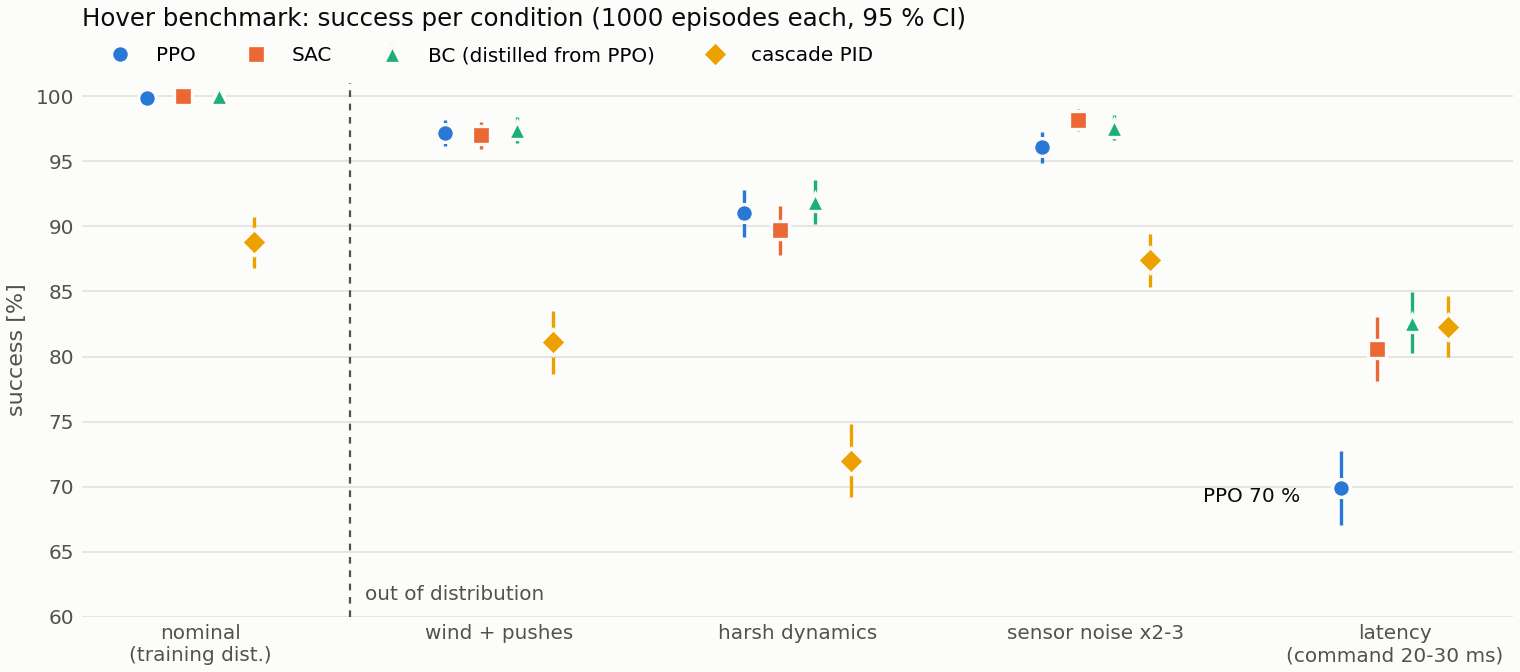
\includegraphics[width=\linewidth]{framework_hover_benchmark.png}
\caption{Hover benchmark suite: success per evaluation condition for PPO, the framework's SAC, a BC student distilled
from the PPO policy and the cascade baseline (1000 episodes per point, same seed, 95\,\% CI; values in
\cref{tab:fw_algos}).}\label{fig:fw_bench}
\end{figure}

\begin{table}[!htbp]\centering\small\caption{Hover benchmark suite: success per condition (1000 episodes each, same seed, fresh process per controller and condition) and generalization gap id$-$mean(ood) in points. Source: \texttt{docs/results/framework/bench\_hover\_algos.json}.}\label{tab:fw_algos}
\begin{adjustbox}{max width=\linewidth}\begin{tabular}{lcccccc}\toprule
Controller & nominal (id) & wind\_push & harsh\_dynamics & sensor\_noise & latency & gap\\\midrule
ppo & 99.9\,\% & 97.2\,\% & 91.0\,\% & 96.1\,\% & 69.9\,\% & +11.4\\
sac & 100.0\,\% & 97.0\,\% & 89.7\,\% & 98.2\,\% & 80.6\,\% & +8.6\\
bc\_distilled & 100.0\,\% & 97.4\,\% & 91.9\,\% & 97.6\,\% & 82.6\,\% & +7.6\\
cascade & 88.8\,\% & 81.1\,\% & 72.0\,\% & 87.4\,\% & 82.3\,\% & +8.1\\
\bottomrule\end{tabular}\end{adjustbox}
\end{table}

\begin{table}[!htbp]\centering\small\caption{Learning algorithms on hover (nominal condition, 1000 episodes). Position error in cm, yaw error in rad. Source: \texttt{offpolicy\_hover.json}.}\label{tab:fw_offpolicy}
\begin{adjustbox}{max width=\linewidth}\begin{tabular}{lcccc}\toprule
Algorithm & Success & Pos. err [cm] & Yaw err [rad] & Train [min]\\\midrule
PPO (rsl\_rl), 4096 envs, 600 it. & 99.9\,\% & 1.26\,$\pm$\,0.04 & 0.08\,$\pm$\,0.00 & --\\
SAC (quadsim), 1024 envs, 15k steps & 100.0\,\% & 1.67\,$\pm$\,0.05 & 0.51\,$\pm$\,0.01 & 21\\
TD3 (quadsim), 1024 envs, 15k steps & 0.0\,\% & 87.49\,$\pm$\,1.77 & 0.63\,$\pm$\,0.02 & 19\\
TD3, noise 0.05-0.15, reward scale 10, 8 upd./step & 99.9\,\% & 2.73\,$\pm$\,0.24 & 1.06\,$\pm$\,0.01 & 28\\
ARS (plugin example), 150 it. & 46.8\,\% & 11.87\,$\pm$\,0.40 & 0.58\,$\pm$\,0.04 & 12\\
\bottomrule\end{tabular}\end{adjustbox}
\end{table}

\begin{table}[!htbp]\centering\small\caption{New vehicles, control interfaces and tasks defined through the extension points (1000 episodes; position error in cm). Source: \texttt{vehicles\_interfaces.json}.}\label{tab:fw_vehicles}
\begin{adjustbox}{max width=\linewidth}\begin{tabular}{lccc}\toprule
Configuration & Success & Pos. err [cm] & Crash\\\midrule
hexa\_x (6 rotors, generated frame), CTBR, PPO & 99.8\,\% & 1.21\,$\pm$\,0.03 & 0.0\,\%\\
hexa\_x, cascade baseline & 96.2\,\% & 4.46\,$\pm$\,0.68 & 0.3\,\%\\
hexa\_x, motor-level (6-D action), PPO & 100.0\,\% & 1.40\,$\pm$\,0.04 & 0.0\,\%\\
x500, acceleration interface (plugin example), PPO & 99.7\,\% & 1.40\,$\pm$\,0.05 & 0.0\,\%\\
landing task (plugin example), PPO, first reward & 0.0\,\% & -- & 0.5\,\%\\
landing task, PPO, reward v2 (time penalty, low-and-slow term) & 94.1\,\% & -- & 5.9\,\%\\
landing task, cascade baseline & 64.1\,\% & -- & 35.9\,\%\\
\bottomrule\end{tabular}\end{adjustbox}
\end{table}

\begin{table}[!htbp]\centering\small\caption{Constrained waypoint racing: speed $\le$\,\SI{2}{m/s}, budget \SI{0.1}{s} of over-speed flight per episode (500 episodes). Source: \texttt{safe\_rl.json}.}\label{tab:fw_safe}
\begin{adjustbox}{max width=\linewidth}\begin{tabular}{lcccc}\toprule
Policy & Success & Episode cost [s] & Time [s] & Crash\\\midrule
PPO (unconstrained) & 99.4\,\% & 5.350\,$\pm$\,0.076 & 6.66\,$\pm$\,0.11 & 0.6\,\%\\
cascade & 91.6\,\% & 6.503\,$\pm$\,0.123 & 10.38\,$\pm$\,0.15 & 2.0\,\%\\
PPO-Lagrangian (PID multiplier) & 87.6\,\% & 0.081\,$\pm$\,0.017 & 11.89\,$\pm$\,0.15 & 0.0\,\%\\
\bottomrule\end{tabular}\end{adjustbox}
\end{table}

\begin{table}[!htbp]\centering\small\caption{Drone racing (2 laps, 7 gates, 5-inch racer); trained on random circuits. Source: \texttt{bench\_race.json}.}\label{tab:fw_race}
\begin{adjustbox}{max width=\linewidth}\begin{tabular}{llcccc}\toprule
Controller & Condition & success & lap\_time & gates\_passed & crash\\\midrule
cascade & random\_tracks (id) & 0.6\,\% & 15.04\,$\pm$\,0.32 & 6.62\,$\pm$\,0.28 & 25.2\,\%\\
cascade & ellipse (ood) & 0.0\,\% & 15.22\,$\pm$\,0.31 & 7.14\,$\pm$\,0.26 & 14.4\,\%\\
cascade & figure8 (ood) & 0.0\,\% & 18.42\,$\pm$\,0.18 & 6.06\,$\pm$\,0.21 & 16.0\,\%\\
cascade & wind (ood) & 0.6\,\% & 15.08\,$\pm$\,0.32 & 6.28\,$\pm$\,0.29 & 27.8\,\%\\
ppo & random\_tracks (id) & 94.4\,\% & 2.47\,$\pm$\,0.02 & 13.49\,$\pm$\,0.20 & 5.6\,\%\\
ppo & ellipse (ood) & 99.6\,\% & 2.49\,$\pm$\,0.01 & 13.96\,$\pm$\,0.06 & 0.4\,\%\\
ppo & figure8 (ood) & 5.4\,\% & 4.15\,$\pm$\,0.05 & 3.40\,$\pm$\,0.39 & 94.6\,\%\\
ppo & wind (ood) & 95.8\,\% & 2.47\,$\pm$\,0.02 & 13.63\,$\pm$\,0.17 & 4.2\,\%\\
ppo\_v1 & random\_tracks (id) & 94.8\,\% & 2.45\,$\pm$\,0.02 & 13.46\,$\pm$\,0.21 & 5.2\,\%\\
ppo\_v1 & ellipse (ood) & 98.0\,\% & 2.49\,$\pm$\,0.01 & 13.84\,$\pm$\,0.10 & 2.0\,\%\\
ppo\_v1 & figure8 (ood) & 73.8\,\% & 3.73\,$\pm$\,0.02 & 12.90\,$\pm$\,0.50 & 26.2\,\%\\
ppo\_v1 & wind (ood) & 95.4\,\% & 2.47\,$\pm$\,0.02 & 13.56\,$\pm$\,0.19 & 4.6\,\%\\
\bottomrule\end{tabular}\end{adjustbox}
\end{table}

\begin{table}[!htbp]\centering\small\caption{Four-agent antipodal swap (shared policy, centralized critic). Source: \texttt{bench\_swarm.json}.}\label{tab:fw_swarm}
\begin{adjustbox}{max width=\linewidth}\begin{tabular}{llcccc}\toprule
Controller & Condition & success & agent\_collision & min\_separation & time\_to\_goal\\\midrule
cascade & swap4 (id) & 35.9\,\% & 36.1\,\% & 0.95\,$\pm$\,0.02 & 2.28\,$\pm$\,0.03\\
cascade & wind (ood) & 29.7\,\% & 36.9\,\% & 0.95\,$\pm$\,0.02 & 2.30\,$\pm$\,0.03\\
cascade & latency (ood) & 35.9\,\% & 33.8\,\% & 0.95\,$\pm$\,0.02 & 2.24\,$\pm$\,0.02\\
ppo & swap4 (id) & 87.5\,\% & 0.4\,\% & 1.39\,$\pm$\,0.02 & 2.04\,$\pm$\,0.04\\
ppo & wind (ood) & 89.8\,\% & 0.8\,\% & 1.37\,$\pm$\,0.02 & 2.09\,$\pm$\,0.06\\
ppo & latency (ood) & 80.5\,\% & 1.2\,\% & 1.38\,$\pm$\,0.02 & 2.16\,$\pm$\,0.07\\
swarm\_potential & swap4 (id) & 100.0\,\% & 0.0\,\% & 1.28\,$\pm$\,0.01 & 6.89\,$\pm$\,0.08\\
swarm\_potential & wind (ood) & 97.7\,\% & 0.0\,\% & 1.29\,$\pm$\,0.01 & 6.80\,$\pm$\,0.07\\
swarm\_potential & latency (ood) & 96.1\,\% & 0.0\,\% & 1.24\,$\pm$\,0.01 & 6.94\,$\pm$\,0.08\\
\bottomrule\end{tabular}\end{adjustbox}
\end{table}

\begin{table}[!htbp]\centering\small\caption{Imitation learning. Hover: RL-to-BC distillation (last column: final position error [cm]). LangNav: success with training / held-out instruction phrasings and wrong-landmark rate (training phrasing). Source: \texttt{imitation.json}.}\label{tab:fw_il}
\begin{adjustbox}{max width=\linewidth}\begin{tabular}{llccc}\toprule
Task & Policy & Success (train phr.) & Success (held-out) & Wrong / pos. err\\\midrule
hover & PPO teacher & 99.9\,\% & -- & 1.26\,$\pm$\,0.04\\
hover & BC student & 99.9\,\% & -- & 1.26\,$\pm$\,0.04\\
hover & BC student, no last action & 100.0\,\% & -- & 1.32\,$\pm$\,0.04\\
langnav (map) & scripted expert (privileged) & -- & 100.0\,\% & --\\
langnav (map) & BC (with last action) & 15.4\,\% & 41.0\,\% & 0.2\,\%\\
langnav (map) & BC, instruction removed & 10.8\,\% & 10.8\,\% & 10.0\,\%\\
langnav (map) & BC, no last action, unknown words averaged in & 81.0\,\% & 30.8\,\% & 0.0\,\%\\
langnav (map) & same policy, unknown words ignored & 81.0\,\% & 58.2\,\% & 0.0\,\%\\
langnav (map) & + DAgger round 1 & 100.0\,\% & 50.8\,\% & 0.0\,\%\\
langnav (map) & + DAgger round 2 & 100.0\,\% & 56.2\,\% & 0.0\,\%\\
langnav (map) & same data, frozen CLIP text encoder & 100.0\,\% & 97.0\,\% & 0.0\,\%\\
langnav (RGB) & scripted expert (privileged) & 100.0\,\% & -- & 0.0\,\%\\
langnav (RGB) & BC, FiLM-CNN + instruction & 82.8\,\% & 85.3\,\% & 0.0\,\%\\
langnav (RGB) & + DAgger round 1 & 100.0\,\% & 100.0\,\% & 0.0\,\%\\
langnav (RGB) & same data, frozen CLIP text encoder & 99.7\,\% & 99.1\,\% & 0.0\,\%\\
langnav (RGB) & VLA adapter: colour servo & 6.6\,\% & 7.2\,\% & 0.0\,\%\\
langnav (RGB) & BC, demonstrations re-collected (camera fix) & 83.8\,\% & 90.9\,\% & 0.0\,\%\\
langnav (RGB) & + DAgger round 1, re-collected & 100.0\,\% & 100.0\,\% & 0.0\,\%\\
langnav (RGB) & SmolVLA fine-tuned, 10 actions per chunk & 19.1\,\% & 19.4\,\% & 50.3\,\%\\
langnav (RGB) & SmolVLA fine-tuned, 50 actions per chunk & 27.2\,\% & 22.2\,\% & 59.7\,\%\\
langnav (RGB) & SmolVLA fine-tuned, re-planned every step & -- & 12.2\,\% & --\\
langnav (RGB) & SmolVLA after 5k of the 10k steps, 10 per chunk & 12.8\,\% & -- & 31.9\,\%\\
langnav (RGB) & SmolVLA, empty instruction, 10 per chunk & 19.7\,\% & -- & 59.4\,\%\\
\bottomrule\end{tabular}\end{adjustbox}
\end{table}

\begin{table}[!htbp]\centering\small\caption{Multi-seed replication: the published single-seed runs (seed 42; BC seed 0) and two more seeds with identical configurations; mean $\pm$ sample std over seeds and a stratified bootstrap 95\,\% CI of the mean over seeds. BC seeds vary initialization and train/validation split on the same demonstrations. Source: \texttt{multiseed.json}.}\label{tab:fw_multiseed}
\begin{adjustbox}{max width=\linewidth}\begin{tabular}{lccccc}\toprule
Result & Seed 42 / 0 & Seed 1 & Seed 2 & Mean $\pm$ std & 95\,\% CI\\\midrule
Race-v0, success [\%], random tracks & 94.4 & 97.2 & 96.8 & 96.1\,$\pm$\,1.5 & [94.4, 97.2]\\
Race-v0, success [\%], ellipse & 99.6 & 99.2 & 98.2 & 99.0\,$\pm$\,0.7 & [98.2, 99.6]\\
Race-v0, success [\%], figure8 & 5.4 & 6.4 & 0.4 & 4.1\,$\pm$\,3.2 & [0.4, 6.4]\\
Race-v0, success [\%], wind & 95.8 & 95.8 & 96.6 & 96.1\,$\pm$\,0.5 & [95.8, 96.6]\\
Race-v1 (both directions), success [\%], random tracks & 94.8 & 96.8 & 95.6 & 95.7\,$\pm$\,1.0 & [94.8, 96.8]\\
Race-v1 (both directions), success [\%], ellipse & 98.0 & 97.2 & 97.2 & 97.5\,$\pm$\,0.5 & [97.2, 98.0]\\
Race-v1 (both directions), success [\%], figure8 & 73.8 & 66.6 & 79.2 & 73.2\,$\pm$\,6.3 & [66.6, 79.2]\\
Race-v1 (both directions), success [\%], wind & 95.4 & 95.4 & 95.8 & 95.5\,$\pm$\,0.2 & [95.4, 95.8]\\
Race-v1, finish terminal, success [\%], random tracks & 90.4 & 95.8 & 94.0 & 93.4\,$\pm$\,2.7 & [90.4, 95.8]\\
Race-v1, finish terminal, success [\%], ellipse & 93.6 & 98.2 & 96.4 & 96.1\,$\pm$\,2.3 & [93.6, 98.2]\\
Race-v1, finish terminal, success [\%], figure8 & 43.0 & 21.6 & 74.2 & 46.3\,$\pm$\,26.5 & [21.6, 74.2]\\
Race-v1, finish terminal, success [\%], wind & 90.6 & 95.6 & 93.0 & 93.1\,$\pm$\,2.5 & [90.6, 95.6]\\
Swarm, success [\%], swap4 & 87.5 & 89.1 & 92.2 & 89.6\,$\pm$\,2.4 & [87.5, 92.2]\\
Swarm, success [\%], wind & 89.8 & 77.3 & 89.1 & 85.4\,$\pm$\,7.0 & [77.3, 89.8]\\
Swarm, success [\%], latency & 80.5 & 76.6 & 72.7 & 76.6\,$\pm$\,3.9 & [72.7, 80.5]\\
Swarm, agent collisions [\%], swap4 & 0.4 & 4.3 & 0.4 & 1.7\,$\pm$\,2.3 & [0.4, 4.3]\\
PPO-Lagrangian, episode cost [s] (budget 0.1) & 0.081 & 0.126 & 0.108 & 0.105\,$\pm$\,0.023 & [0.081, 0.126]\\
PPO-Lagrangian, success [\%] & 87.6 & 0.0 & 85.2 & 57.6\,$\pm$\,49.9 & [0.0, 87.6]\\
LangNav map, BC, unknown words averaged, success [\%], train phr. & 81.0 & 68.8 & 78.0 & 75.9\,$\pm$\,6.4 & [68.8, 81.0]\\
LangNav map, BC, unknown words averaged, success [\%], held-out phr. & 30.8 & 15.6 & 14.4 & 20.3\,$\pm$\,9.1 & [14.4, 30.8]\\
LangNav map, BC, success [\%], train phr. & 81.0 & 68.8 & 78.0 & 75.9\,$\pm$\,6.4 & [68.8, 81.0]\\
LangNav map, BC, success [\%], held-out phr. & 58.2 & 64.0 & 62.4 & 61.5\,$\pm$\,3.0 & [58.2, 64.0]\\
LangNav map, DAgger-2, success [\%], train phr. & 100.0 & 100.0 & 100.0 & 100.0\,$\pm$\,0.0 & [100.0, 100.0]\\
LangNav map, DAgger-2, success [\%], held-out phr. & 56.2 & 84.2 & 80.0 & 73.5\,$\pm$\,15.1 & [56.2, 84.2]\\
LangNav map, DAgger-2 + CLIP, success [\%], train phr. & 100.0 & 100.0 & 100.0 & 100.0\,$\pm$\,0.0 & [100.0, 100.0]\\
LangNav map, DAgger-2 + CLIP, success [\%], held-out phr. & 97.0 & 95.6 & 98.0 & 96.9\,$\pm$\,1.2 & [95.6, 98.0]\\
LangNav RGB, BC, success [\%], train phr. & 82.8 & 75.3 & 71.9 & 76.7\,$\pm$\,5.6 & [71.9, 82.8]\\
LangNav RGB, BC, success [\%], held-out phr. & 85.3 & 75.3 & 62.8 & 74.5\,$\pm$\,11.3 & [62.8, 85.3]\\
LangNav RGB, DAgger-1, success [\%], train phr. & 100.0 & 100.0 & 100.0 & 100.0\,$\pm$\,0.0 & [100.0, 100.0]\\
LangNav RGB, DAgger-1, success [\%], held-out phr. & 100.0 & 95.3 & 100.0 & 98.4\,$\pm$\,2.7 & [95.3, 100.0]\\
LangNav RGB, DAgger-1 + CLIP, success [\%], train phr. & 99.7 & 100.0 & 99.7 & 99.8\,$\pm$\,0.2 & [99.7, 100.0]\\
LangNav RGB, DAgger-1 + CLIP, success [\%], held-out phr. & 99.1 & 99.7 & 100.0 & 99.6\,$\pm$\,0.5 & [99.1, 100.0]\\
LangNav RGB, re-collected data, BC, success [\%], train phr. & 83.8 & 83.8 & 73.1 & 80.2\,$\pm$\,6.1 & [73.1, 83.8]\\
LangNav RGB, re-collected data, BC, success [\%], held-out phr. & 90.9 & 82.8 & 59.1 & 77.6\,$\pm$\,16.6 & [59.1, 90.9]\\
LangNav RGB, re-collected data, DAgger-1, success [\%], train phr. & 100.0 & 100.0 & 99.4 & 99.8\,$\pm$\,0.4 & [99.4, 100.0]\\
LangNav RGB, re-collected data, DAgger-1, success [\%], held-out phr. & 100.0 & 100.0 & 97.5 & 99.2\,$\pm$\,1.4 & [97.5, 100.0]\\
\bottomrule\end{tabular}\end{adjustbox}
\end{table}

\begin{table}[!htbp]\centering\small\caption{Comparisons over seeds (Agarwal et al.~\cite{agarwal2021precipice}): probability that a random seed of X beats a random seed of Y on a random condition, and the interquartile mean of the success rate [\%], each with a stratified bootstrap 95\,\% CI. Source: \texttt{multiseed.json} (\texttt{comparisons}).}\label{tab:fw_compare}
\begin{adjustbox}{max width=\linewidth}\begin{tabular}{lccc}\toprule
Comparison X vs Y & P(X $>$ Y) & IQM X & IQM Y\\\midrule
Race v1 vs v0, figure-8 & 1.00 [1.00, 1.00] & 73.2 [66.6, 79.2] & 4.1 [0.4, 6.4]\\
Race v1 vs v0, all 4 conditions & 0.38 [0.25, 0.53] & 95.6 [95.2, 96.2] & 96.1 [95.2, 96.7]\\
Race v1, finish terminal vs time-out, all 4 conditions & 0.25 [0.06, 0.50] & 92.9 [91.4, 94.6] & 95.6 [95.2, 96.2]\\
LangNav map, CLIP vs bag of words (held-out phr.) & 1.00 [1.00, 1.00] & 96.9 [95.6, 98.0] & 73.5 [56.2, 84.2]\\
LangNav map, unknown words ignored vs averaged & 1.00 [1.00, 1.00] & 61.5 [58.2, 64.0] & 20.3 [14.4, 30.8]\\
LangNav RGB, DAgger-1 vs BC (both phrasings) & 1.00 [1.00, 1.00] & 100.0 [97.7, 100.0] & 76.3 [69.6, 82.2]\\
LangNav RGB BC, re-collected vs stale-frame data & 0.67 [0.33, 1.00] & 80.9 [69.6, 85.5] & 76.3 [69.6, 82.2]\\
LangNav RGB DAgger-1, re-collected vs stale-frame data & 0.44 [0.17, 0.67] & 99.8 [98.8, 100.0] & 100.0 [97.7, 100.0]\\
\bottomrule\end{tabular}\end{adjustbox}
\end{table}

\begin{table}[!htbp]\centering\small\caption{Extension examples executed in the simulator (\texttt{examples\_check.py}); success of the classical baseline where the check is an evaluation.}\label{tab:fw_examples}
\begin{adjustbox}{max width=\linewidth}\begin{tabular}{lcc}\toprule
Example & Result & Baseline success\\\midrule
vehicle\_yaml\_hexa & pass & 95\,\%\\
vehicle\_yaml\_inherit & pass & 52\,\%\\
vehicle\_plugin\_quad250 & pass & 61\,\%\\
sensor\_gnss & pass & --\\
task\_landing & pass & --\\
task\_landing\_baseline & pass & 58\,\%\\
reward\_curriculum & pass & --\\
action\_interface\_accel & pass & --\\
algorithm\_ars & pass & --\\
vla\_adapter\_color\_servo & pass & 7\,\%\\
sensor\_lidar\_nav & pass & 43\,\%\\
\bottomrule\end{tabular}\end{adjustbox}
\end{table}



\subsection{Findings}
All numbers below are the values re-measured after the review (\cref{sec:review}); racing, the swarm, the Lagrangian
and the language tasks are given over three seeds.
\begin{itemize}
\item \textbf{Algorithms (\cref{tab:fw_offpolicy,tab:fw_algos,fig:fw_bench}).} With the changes above SAC matches
PPO's in-distribution hover success ($\approx$100\,\%) in 21 instead of 8 minutes, with a slightly larger position error and a
much larger yaw error (its entropy term makes it indifferent to the weakly rewarded yaw). Out of distribution, PPO is
the most sensitive to latency beyond its training range (70\,\% vs 81--83\,\% for SAC and the BC student), so the
benchmark exposes a property that the in-distribution number hides. TD3 with the SAC configuration did not learn;
with smaller exploration noise, a smaller reward scale and 8 updates per step it reaches 99.9\,\%. A plug-in Augmented
Random Search (linear policy) reaches 46.8\,\% in 12 minutes.
\item \textbf{Generality (\cref{tab:fw_vehicles}).} A six-rotor vehicle generated from a frame description trains to
99.8\,\% with the unchanged task, and the extension examples (vehicle files, sensor terms, a new task, a new control
interface, a new algorithm) run through the unmodified scripts.
\item \textbf{Racing (\cref{tab:fw_race,tab:fw_multiseed}).} PPO completes two laps on $96\pm2$\,\% of unseen random
circuits at \SI{11.9}{m/s} mean speed (\SI{2.5}{s} per lap), transfers to a fixed reference circuit and to wind, but
rarely completes the figure-8 ($4\pm3$\,\%): the training circuits only turn counter-clockwise, the figure-8
alternates directions. Retraining with half of the circuits mirrored (both turning directions, same budget) raises the
figure-8 completion to $73\pm6$\,\% while keeping 95--98\,\% elsewhere --- the benchmark located the gap, a one-line
change of the training distribution closed most of it.
The classical cascade with gate-aligned waypoints passes about 7 of 14 gates in the episode (15\,s per lap, 25\,\%
crashes); its first version (straight to the gate centre) crashed into the frames in 99\,\% of the episodes.
\item \textbf{Multi-agent (\cref{tab:fw_swarm}).} The shared PPO policy coordinates four agents through the
antipodal swap (agent collisions 36\,\% for uncoordinated straight lines, $1.7\pm2.3$\,\% for PPO) and is 3.4 times
faster than a tuned potential field, which is, however, more reliable (100 vs $89.6\pm2.4$\,\% group success). The potential field's
gains were selected on the training scenario after its first setting failed (0\,\%, 53\,\% collisions).
\item \textbf{Constraints (\cref{tab:fw_safe,tab:fw_multiseed}).} The Lagrangian keeps the over-speed time around its
budget ($0.105\pm0.023$ vs \SI{0.1}{s} over three seeds) while the unconstrained policy spends \SI{5.4}{s} per course
above the limit; the price is a slower course and, in one of three seeds, a policy that never learned to finish the
course: its multiplier grew to $\approx$5 within 150 iterations, before the task was learned.
\item \textbf{Imitation and language (\cref{tab:fw_il}).} An RL policy distils into a BC student without loss. For
language-conditioned navigation, the last-action input makes BC copy its previous command and fail to stop (causal
confusion~\cite{dehaan2019causal}); removing it and two DAgger rounds reach the expert's 100\,\%. A bag-of-words
instruction encoder generalizes to unseen phrasings only if unknown words are ignored ($62\pm3$ vs $20\pm9$\,\% on the
same checkpoints) and then reaches $74\pm15$\,\% after DAgger, whereas a frozen pretrained CLIP text tower, with the
same data and policy, reaches $96.9\pm1.2$\,\%. With the RGB camera instead of the
landmark map (colours grounded in pixels), the FiLM-CNN policy reaches $77\pm6$\,\% and, after one DAgger round,
100\,\% (held-out phrasings $98\pm3$\,\%); its failures before DAgger were almost all collisions while approaching
(a wrong pillar in 1 of 320 episodes). A model-free colour-servo adapter exercises the VLA interface (7\,\%: correct
pillar, stopping rule outside the success zone).
\item \textbf{Defects found by the checks.} The example check found that observation terms were evaluated before
task buffers existed (now set up after the most-derived constructor) and that non-directory checkpoints (VLA
factories) were mistaken for run directories; a crashed simulator process hung for minutes holding GPU memory
(scripts now terminate after an exception). Demonstration collection stopping at a global episode count would bias
datasets toward short episodes (now a per-environment quota) --- the same stopping rule remained in the evaluator until
the review (\cref{sec:review}). The regression check was re-run after these fixes.
\end{itemize}

\subsection{Review, corrections and multi-seed replication}\label{sec:review}
\paragraph{Procedure.} After the framework milestone the code base was reviewed by three independent reviewers (one
for the core, vehicles, control interfaces and export; one for the task environments, terms and baselines; one for
the learning algorithms, imitation learning, evaluation and result tooling), each without access to the others'
findings, and the documentation was checked mechanically (every referenced file and task exists). Every reported
defect was reproduced before it was fixed --- on the CPU wherever possible, with a unit test that fails on the previous
code and passes after the fix (124 $\to$ 141 tests). The fixes were developed in a separate checkout while the
multi-seed training queue kept running on the unchanged code, so that all seeds of a task were trained with the same
code. \Cref{tab:review} lists the defects and their effect on published results.

\begin{table}[!htbp]\centering\small
\caption{Defects found by the review (effect on the results published before it, and the fix).}\label{tab:review}
\begin{tabularx}{\linewidth}{>{\raggedright\arraybackslash}X>{\raggedright\arraybackslash}p{0.27\linewidth}>{\raggedright\arraybackslash}p{0.2\linewidth}}\toprule
Defect & Effect on published results & Fix\\\midrule
Evaluator stopped at a global episode count and kept every finished episode: the episodes still running (the long
ones) were dropped & every evaluation; largest where outcomes differ in episode length & per-environment quota,
everything re-measured\\
Cascade baseline: velocity integrator not reset between episodes & cascade on hover, tracking, waypoints, racing &
reset per episode\\
Initial angular velocity written to PhysX in the world frame but used as a body rate by gyro, odometry and rate loop &
hover (first steps of an episode) & body-frame sample, rotated for PhysX\\
SAC Polyak-averaged its target critic twice per gradient step & published SAC run used $\tau_\text{eff}=0.00998$
(configuration said 0.005) & one update, default $\tau=0.01$\\
Off-policy resume acted randomly while refilling the replay buffer & none & policy refills the buffer\\
Curriculum averaged the last episode of every environment (mostly easier levels) and ran away & example only & judge
each level on its own episodes\\
Mixer used an equal collective split also for asymmetric layouts (torque at every thrust level) & none (presets
symmetric) & zero-torque split\\
\texttt{--plugins m.py env.a=b}: argparse attached the override to the plugin list & documented commands failed &
overrides recovered\\
Vehicle files: \texttt{1e-5} read as a string, invalid spins, \texttt{k\_f} together with thrust-to-weight, CoM
outside the rotor polygon accepted & none & typed parsing, validation\\
Hardware check counted the simulator's own memory twice & seed-42 safe-RL run used 3456 instead of 4096 environments &
own memory added back\\
Export: no plugins or overrides, exported network not taken from the algorithm, position contract incomplete & plug-in
tasks not exportable & completed\\
Result collector would have read the multi-seed tag as the curated race/swarm table; stale benchmark results reused
after a failure & latent & fixed sources, stale files removed\\
Rendered cameras: first frame of every episode showed the previous scene & RGB demonstrations ($\approx$0.7\,\% stale
frames) & re-render after resets\\
Race: 6.2\,\% of random circuits had overlapping gates, 0.22\,\% started inside a gate frame & random-circuit
conditions & resampled\\
LangNav: a dwell completed in a collision step counted as success and crash & 2 of 500 episodes & exclusive\\
Minor: unbounded cost list without Lagrangian, multiplier integral wind-up, silent reward-term override, ignored
\texttt{speed\_limit} override, BC on tiny datasets & none & fixed\\
\bottomrule\end{tabularx}
\end{table}

\paragraph{Evaluation sampling bias.} The evaluator ran $N$ parallel environments until the number of finished
episodes reached the requested $E$ and kept all of them. With $k=E/N\approx2$ episodes per environment this is a biased
sample: an environment whose episodes end early (a crash, an early success) contributes more of them, and the
episodes still running at the stopping time --- by the inspection paradox, preferentially the long ones --- are
discarded. Outcomes that end episodes early are therefore over-represented. In the extreme, the counter-clockwise
racing policy was reported at 0\,\% on the figure-8 because its few successful two-lap episodes ($\approx$\SI{7.4}{s})
had not finished when the crashed environments ($\approx$\SI{1}{s}) had produced the requested count. The corrected
evaluator takes the first $k=\lceil E/N\rceil$ episodes of every environment, which is unbiased because the
inclusion of an episode no longer depends on its length (the demonstration collector already used this rule). All
127 published evaluations (and 28 of the replication) were re-run from their recorded metadata; the median change of a success rate is 0.4
points, the largest are listed in \cref{tab:reeval}.

\paragraph{Regression evidence.} On the 59 reference metrics, the corrected evaluator alone leaves hover and tracking
unchanged (their episodes end together at the time limit) and changes navigation and the waypoint cascade; the
other fixes on top change exactly the metrics they act on (hover PPO and cascade through the reset frame, the
cascade on tracking and waypoints through the integrator reset) and leave the tracking, waypoint and navigation
policies and the SE(3) and potential-field baselines bit-identical.

\begin{table}[!htbp]\centering\small
\caption{Published vs.\ corrected values (largest changes; full record in
\texttt{docs/results/framework/reevaluation.json}).}\label{tab:reeval}
\begin{tabular}{lcc}\toprule
Result & Published & Corrected\\\midrule
Racing v0, figure-8 success & 0\,\% & 5.4\,\% \\
Racing v1 (both directions), figure-8 success & 54.3\,\% & 73.8\,\% \\
Racing cascade, crashes (random circuits) & 40\,\% & 25\,\% \\
Swarm, straight lines: success / collisions & 18.3 / 44.6\,\% & 35.9 / 36.1\,\% \\
Range navigation: PPO / potential field & 83.0 / 49.8\,\% & 84.4 / 39.4\,\% \\
Landing cascade success & 52.0\,\% & 64.1\,\% \\
LangNav BC with last action, held-out phrasing & 20.4\,\% & 41.0\,\% \\
LangNav DAgger-2 (bag of words) / CLIP, held-out & 59.7 / 99.8\,\% & 56.2 / 97.0\,\% \\
Hover cascade, nominal / wind + pushes & 88.7 / 78.6\,\% & 90.3 / 80.8\,\% \\
\bottomrule\end{tabular}
\end{table}

\paragraph{Multi-seed replication.} Racing, the multi-agent swap, PPO-Lagrangian and the language-conditioned
imitation policies were re-trained with two further seeds (identical code and configuration;
\cref{tab:fw_multiseed}). Training on both turning directions raises figure-8 completion from $4\pm3$ to
$73\pm6$\,\%; the shared swarm policy reaches $89.6\pm2.4$\,\% group success. The Lagrangian keeps the over-speed time
around its budget ($0.105\pm0.023$\,s for a 0.1\,s budget), but one of three seeds never learned to finish the course:
its multiplier grew while the policy was still learning the task. Ignoring unknown words in the bag-of-words encoder
raises held-out-phrasing success from $20\pm9$ to $62\pm3$\,\% on the same checkpoints, and a frozen CLIP text tower
reaches $96.9\pm1.2$\,\% against $73.5\pm15.1$\,\% for the bag of words after two DAgger rounds.

\subsection{Tools for VLA research and rigorous reporting}\label{sec:tools}
\paragraph{Remote policies.} Vision-language-action models are usually evaluated behind a policy server in their own
environment: openpi's server (used for $\pi_0$~\cite{black2024pi0}) answers observation dictionaries sent over a
WebSocket with msgpack-encoded numpy arrays, and Isaac Lab-Arena and BEHAVIOR evaluate models through the same
interface. quadsim implements this protocol on both sides: a client adapter that queries the server (camera image as
uint8 HWC or exact float, proprioception, the full deployable observation and the instruction; the first $k$ actions
of a returned chunk are executed open loop, as openpi's action-chunk broker, and a new episode starts with a fresh
chunk) and servers for quadsim checkpoints, for any LeRobot policy trained on a quadsim export (with the policy's own
pre- and post-processing) and for arbitrary \texttt{infer(obs)} functions. A behaviour-cloning policy evaluated through a separate server process reproduces the
local closed-loop evaluation bit for bit (every metric of 500 LangNav episodes), and a server in the LeRobot
environment (NumPy~2) exchanges arrays exactly with the simulator's client (NumPy~1.26), so models with incompatible
dependencies can be benchmarked on the drone tasks unchanged.

\paragraph{Statistics and datasets.} Multi-seed results are aggregated with the metrics recommended by Agarwal et
al.~\cite{agarwal2021precipice} (interquartile mean, stratified bootstrap confidence intervals over seeds, probability of
improvement; \cref{tab:fw_compare}). They make one nuance explicit that the means hide: training the racing policy on
both turning directions wins on the figure-8 with probability 1.00 but only 0.38 over all four conditions, because
it loses 0.4--1.5 points on the others. Exported LeRobot datasets carry a Hugging Face dataset card (features,
provenance, verification, limitations), and the repository provides a benchmark protocol, a citation file, a licence
file, a changelog and contribution rules.

\paragraph{Constraint warm-up and budget curriculum.} To address the PPO-Lagrangian seed that never learned the course,
two variants were trained (seed 42): a 300-iteration unconstrained warm-up, and the same warm-up followed by a budget
that shrinks geometrically from 5 to \SI{0.1}{s} over 600 iterations. Both failed (course success 2.0 and 1.2\,\%,
over-speed 1.26 and \SI{1.22}{s} per course, against 87.6\,\% and \SI{0.081}{s} without them): the warm-up policy
races with $\approx$\SI{5.5}{s} of over-speed per course, its over-speed time barely decreases once the constraint
acts, the multiplier saturates at its maximum and the task collapses. In this reward-penalty form a converged policy
is not steered back to the constraint; enforcing it from the start works in two of three seeds, and a separate cost
critic is the next step.

\paragraph{Terminal task ends.} The goal-reaching tasks return a reached goal or a finished course as a time-out, so
the learners bootstrap the value of the final state. The option \texttt{task\_end\_is\_terminal} makes these ends
terminal. On Race-v1 (three seeds each, identical configuration and budget) the terminal variant is worse: success
$93.4\pm2.7$ vs.\ $95.7\pm1.0$\,\% on random circuits and $46\pm26$ vs.\ $73\pm6$\,\% on the figure-8, a
probability of improvement of 0.25 [0.06, 0.50] over the four conditions (\cref{tab:fw_compare}), with slower laps
(3.0 vs.\ \SI{2.5}{s}) and more crashes (6.6 vs.\ 4.3\,\% in distribution). The bootstrapped value at the finish
acts as an additional incentive to reach it early; the published formulation is kept.

\paragraph{Re-collected RGB demonstrations.} After the camera fix the RGB demonstrations were collected again (the
same 297\,675 transitions; only the first image of every episode differs) and BC and one DAgger round re-trained
with three seeds: $80.2\pm6.1$ vs.\ $76.7\pm5.6$\,\% for BC on the training phrasings (probability of improvement
0.67 [0.33, 1.00]) and $99.8$ vs.\ $100$\,\% after DAgger. The stale frame had no measurable effect.

\paragraph{A pretrained VLA on the drone task.} SmolVLA~\cite{shukor2025smolvla} (450\,M parameters, a
flow-matching action expert on a truncated SmolVLM2) was fine-tuned with LeRobot's recipe (frozen vision encoder;
10\,k steps of 32 samples, 1.07 epochs, \SI{86}{min} on the RTX~5060) on the re-collected demonstrations and
evaluated through the policy server with the BC protocol (\cref{tab:fw_il}). It flies to a pillar but picks the
instructed one at chance level: 19\,\% success executing 10 actions per chunk (27\,\% with 50, 12\,\% re-planning
every step), 45--66\,\% wrong pillar among four, against 80\,\% for the FiLM-CNN behaviour cloning trained from
scratch on the same data. Once the vehicle moves, changing the colour word alters its actions by at most 0.03: it
continues the motion in its own velocity estimate, the copycat shortcut of behaviour
cloning~\cite{dehaan2019causal}. At the first frame its actions depend on the colour word through a fixed
colour-to-direction prior rather than on where the colour is in the image (turn direction agrees with the expert in
44\,\% of the episodes, chance 50\,\%). Training longer improves the flight but not the choice: from 5\,k to
10\,k steps the crashes fall from 54 to 29\,\% while the share of pillar arrivals at the instructed pillar stays
at 28--29\,\% (chance 25\,\%), and with an empty instruction the policy succeeds as often as with it (19.7 vs.\
19.1\,\%). One fine-tuning run on $48\times64$ images is not a
verdict on VLAs, but the benchmark separates flight competence from instruction grounding, and the toolchain
(export, LeRobot fine-tuning, policy server, closed-loop evaluation) is in place for stronger models.
